\section{Derivations and exactness boundary}

\subsection{Proof of Proposition 1: necessity of the cross statistic}
\label{app:cross-necessity}

Let $S$ denote the retained summary and assume a zero-error decoder
$D(S,h_u(\beta_0),\Delta)=h_u(\beta_0+\Delta)$ for every admissible
$\Delta$. Equation~(\ref{eq:stale}) then implies
\[
 h_u(\beta_0)-D(S,h_u(\beta_0),\Delta)=R_{u\beta}\Delta.
\]
The retained information therefore determines the action of $R_{u\beta}$ on the
span of admissible changes. If this span is $\mathbb R^{d_\beta}$, evaluating
the decoder on a basis recovers every column of $R_{u\beta}$. Conversely,
retaining $R_{u\beta}$ makes the correction explicit through
Eq.~(\ref{eq:stale}). Two historical datasets with the same retained summary
but different actions $R_{u\beta}\Delta$ would require the decoder to return
different values from identical inputs, contradicting error-free recovery.

\subsection{Proof of Proposition 2: historical likelihood-factor transfer}
\label{app:joint-transfer}

Conditionally write $u_o=L_{on}u_n+\delta$ with $\E[\delta\mid u_n]=0$. For $z_o=M_{on}z_n+[0,\delta]^{\trans}$, substitution into Eq.~(\ref{eq:old-like}) followed by conditional expectation gives
\[
 -\tfrac12 z_n^{\trans}M_{on}^{\trans}R_oM_{on}z_n
 +r_o^{\trans}M_{on}z_n
 -\tfrac12\operatorname{tr}(R_{uu,o}\operatorname{Cov}(\delta)).
\]
The trace is constant in $(\beta,u_n)$, leaving Eq.~(\ref{eq:transfer}). The transferred cross block is therefore $R_{\beta u,o}L_{on}$. This establishes a one-step projected log factor and does not compare the resulting posterior with a full-history posterior expressed in the current inducing representation.

\subsection{Proof of Proposition 3: one-step projection optimality and loss}
\label{app:transfer-proof}

Write $u_o=m+\delta$, where $m=L_{on}u_n$ and, conditional on $(\beta,u_n)$, $\delta\sim\mathcal N(0,\Sigma_{o\mid n})$. Expanding the terms that depend on $\delta$ gives
\begin{align*}
 g(\beta,m+\delta)&=c(\beta,u_n)+a^{\trans}\delta
 -\tfrac12\delta^{\trans}R_{uu}\delta,\\
 a&=r_u-R_{u\beta}\beta-R_{uu}m.
\end{align*}
After centring,
\[
 g-\E[g\mid\beta,u_n]
 =a^{\trans}\delta-\tfrac12\{\delta^{\trans}R_{uu}\delta-
 \operatorname{tr}(R_{uu}\Sigma_{o\mid n})\}.
\]
The cross covariance vanishes because centred Gaussian third moments are zero. The linear term has variance $a^{\trans}\Sigma_{o\mid n}a$, while the unscaled quadratic term has variance $2\operatorname{tr}[(R_{uu}\Sigma_{o\mid n})^2]$. This gives Eq.~(\ref{eq:transfer-mse}), and optimality follows because conditional expectation is the orthogonal projection in $L^2$. Finally,
$a^{\trans}\Sigma a\leq\|\Sigma\|_2\|a\|_2^2$ and
$\operatorname{tr}[(R\Sigma)^2]=\|\Sigma^{1/2}R\Sigma^{1/2}\|_F^2\leq\|R\|_F^2\|\Sigma\|_2^2$.

For the nested-space statement, the conditional mean is again an $L^2$ projection. Its squared reconstruction error is the trace of the conditional covariance, and the Pythagorean theorem for nested projection subspaces makes this error non-increasing. This statement requires both the old target and its joint law to remain fixed; unrelated feature families at different $M_t$ need not be nested.

\subsection{Proof of Proposition 4: single-Kronecker likelihood invariant}
\label{app:kron-invariant}

Under separability and unchanged spatial functionals,
$K_{k-1,k}=K_{k-1,k}^{(t)}\otimes K_s$ and
$K_{k,k}=K_{k,k}^{(t)}\otimes K_s$. Hence
\begin{align*}
L_{k-1,k}&=K_{k-1,k}K_{k,k}^{-1}\\
&=\{K_{k-1,k}^{(t)}(K_{k,k}^{(t)})^{-1}\}\otimes I_{M_s}\\
&=L_t\otimes I_{M_s}.
\end{align*}
If $R_{uu,k-1}=B_{k-1}\otimes G$, conditional transport gives
\[
(L_t\otimes I)^{\trans}(B_{k-1}\otimes G)(L_t\otimes I)
=(L_t^{\trans}B_{k-1}L_t)\otimes G.
\]
For a Cartesian block, $A_k=P_{t,k}\otimes C$ and therefore
\[
\sigma_y^{-2}A_k^{\trans}A_k
=(\sigma_y^{-2}P_{t,k}^{\trans}P_{t,k})\otimes(C^{\trans}C).
\]
With $G=C^{\trans}C$, their sum is precisely $B_k\otimes G$. The base case
$B_0=0$, followed by induction over blocks, establishes Proposition~\ref{prop:kron-invariant}.

\subsection{Proof of Lemma 1: structured Sylvester solve for the inducing-variable precision block}
\label{app:sylvester-proof}

Under the column-major vectorisation convention,
$(A\otimes B)\operatorname{vec}(Z)=\operatorname{vec}(BZA^{\trans})$.
Applying this identity to the two terms in Eq.~(\ref{eq:du-operator}) gives
Eq.~(\ref{eq:sylvester}). Substitute

\begin{equation*}
 Z=K_s^{1/2}\widetilde ZK_{t,k}^{1/2}
\end{equation*}

and multiply by the corresponding square roots. This gives
\begin{align*}
\widetilde Z+\widetilde G\,\widetilde Z\,\widetilde B&=\widetilde Q,
\end{align*}
where
\begin{equation*}
\begin{aligned}
\widetilde G&=K_s^{1/2}GK_s^{1/2},\qquad
\widetilde B=K_{t,k}^{1/2}B_kK_{t,k}^{1/2},\\
\widetilde Q&=K_s^{1/2}QK_{t,k}^{1/2}.
\end{aligned}
\end{equation*}
Let
\[
\widetilde G=U_s\operatorname{diag}(\gamma_i)U_s^{\trans},\qquad
\widetilde B=U_t\operatorname{diag}(\eta_j)U_t^{\trans},
\]
and define
\[
\widehat Z=U_s^{\trans}\widetilde ZU_t,\qquad
\widehat Q=U_s^{\trans}\widetilde Q U_t.
\]
Writing $\widetilde Z=U_s\widehat ZU_t^{\trans}$ and rotating by these
eigensystems gives
$(1+\gamma_i\eta_j)\widehat Z_{ij}=\widehat Q_{ij}$.
Positive semidefiniteness implies $1+\gamma_i\eta_j\geq1$, establishing
Eq.~(\ref{eq:sylvester-solution}) and uniqueness. The recovered matrix is
$\widetilde Z=U_s\widehat ZU_t^{\trans}$ followed by
$Z=K_s^{1/2}\widetilde ZK_{t,k}^{1/2}$.

\subsection{Proof of Theorem 1: dense equivalence of the transferred finite-dimensional target}
\label{app:dense-equivalence}

Proposition~\ref{prop:kron-invariant} gives the lower-right block
$D_u$ of the densely assembled transferred precision. Lemma~\ref{lem:sylvester}
replaces each application of $D_u^{-1}$ with an algebraically equivalent structured matrix
solve, after which the standard Schur-complement block inverse is applied to the
same $\Lambda_k$. Define the Schur complement
\[
P_\beta=A_\beta-B_{\beta u}D_u^{-1}B_{\beta u}^{\trans}.
\]
Then
\[
S_{\beta\beta}=P_\beta^{-1},\qquad
S_{\beta u}=-P_\beta^{-1}B_{\beta u}D_u^{-1},
\]
\[
S_{uu}=D_u^{-1}+D_u^{-1}B_{\beta u}^{\trans}
P_\beta^{-1}B_{\beta u}D_u^{-1}.
\]
These are precisely the blocks of $\Lambda_k^{-1}$, so the posterior means and
covariance quadratic forms agree with the dense posterior solve. Adding the same full-GP
conditional residual to both predictive variances preserves this equality. Any
remaining difference arises only from finite-precision arithmetic and the same
declared jitter; the structured solve introduces no additional posterior approximation.

\subsection{Prediction with the full conditional}

Let $a_*$ denote the conditional-mean projection row, $h_*=[\phi_*^{\trans},a_*^{\trans}]^{\trans}$, and let $S_k$ be the joint variational covariance. The predictive moments are
\begin{align}
 \E[y_*]&=\phi_*^{\trans}m_\beta+a_*^{\trans}m_u,\\
 \operatorname{Var}(y_*)&=\sigma_y^2+h_*^{\trans}S_kh_*+\nu_*,
 \qquad
 \nu_*=k_{**}-a_*^{\trans}K_ua_*.
\end{align}
The $\nu_*$ term is the GP conditional variance term and is distinct from the VFE trace correction used during hyperparameter calibration.

\subsection{Detailed posterior-solve cost}
\label{app:complexity}
A dense inducing-variable precision factorisation costs $O(M_s^3M_t^3)$ time and
$O(M_s^2M_t^2)$ memory. Accounting for the $d_\beta$ cross-block right-hand
sides and the Schur complement, structured posterior solve costs
\begin{multline}
 O\!\left(M_s^3+M_t^3+(d_\beta+1)
 (M_s^2M_t+M_sM_t^2)\right.\\
 \left.{}+d_\beta^2M_sM_t+d_\beta^3\right),
 \label{eq:recovery-cost}
\end{multline}
and the persistent state occupies
\begin{equation}
 O(M_s^2+M_t^2+(d_\beta+1)M_sM_t+d_\beta^2),
 \label{eq:state-cost}
\end{equation}
for fixed budgets, independently of the number of elapsed blocks. These expressions
cover core posterior computation and persistent state, and exclude current-block
statistic formation, data loading, Task-1 calibration, and all-point prediction.

\section{Experimental protocols}

\subsection{Evaluation metrics}

For $N$ held-out predictions with Gaussian posterior
$y_i\sim\mathcal N(\mu_i,\sigma_i^2)$, define
$z_i=(y_i-\mu_i)/\sigma_i$.  We report
\begin{align}
\operatorname{RMSE}
&=\left[\frac{1}{N}\sum_{i=1}^{N}(y_i-\mu_i)^2\right]^{1/2},
\\
\operatorname{NLPD}
&=\frac{1}{N}\sum_{i=1}^{N}
\left[\frac{1}{2}\log(2\pi\sigma_i^2)
+\frac{(y_i-\mu_i)^2}{2\sigma_i^2}\right],
\\
\operatorname{CRPS}_i
&=\sigma_i\left[z_i\{2\Phi(z_i)-1\}
+2\phi(z_i)-\frac{1}{\sqrt{\pi}}\right],
\\
\operatorname{CRPS}
&=\frac{1}{N}\sum_{i=1}^{N}\operatorname{CRPS}_i,
\end{align}
where $\Phi$ and $\phi$ denote the standard-normal distribution and density.
Calibration is measured over the central predictive intervals
$\mathcal A=\{0.05,0.15,\ldots,0.95\}$:
\begin{align}
\widehat C(\alpha)
&=\frac{1}{N}\sum_{i=1}^{N}
\mathbf{1}\!\left(
|y_i-\mu_i|\leq
\Phi^{-1}\!\left(\frac{1+\alpha}{2}\right)\sigma_i
\right),
\\
\operatorname{ECE}
&=\frac{1}{|\mathcal A|}\sum_{\alpha\in\mathcal A}
|\widehat C(\alpha)-\alpha|.
\end{align}
All four metrics are lower-is-better.  Tables report the mean and sample
standard deviation across the archived spatial splits.  For archived
sample-based predictive distributions, the same central-interval definition
is evaluated using empirical predictive quantiles.

For the ERA5-Land and PEMS-BAY mechanism suites, complete mean $\pm$ sample
SD results, including Coverage90, are reported in Appendix Table~\ref{tab:mechanism_full}.

\FloatBarrier
\subsection{Dataset and protocol overview}

Table~\ref{app:dataset-overview} summarises the spatial units, temporal stream,
information boundary, and role of each dataset. Dataset-specific figures are
shown in the corresponding sections to keep each visual legible at print size.

\begin{table}[H]
\centering
\caption{Dataset and strict-online protocol overview.}
\label{app:dataset-overview}
\scriptsize
\setlength{\tabcolsep}{0.7pt}
\begin{tabular}{@{}lllll@{}}
\toprule
Dataset & Units & Stream & V / H & Domain \\
\midrule
ERA5-Land & 1,000 UK & 171 blk. & 800/200 & Environmental \\
COVID & 52 juris. & 143 wk. & 42/10 & Public health \\
PEMS & 325 sens. & 5-min & 260/65 & Traffic \\
\bottomrule
\end{tabular}
\end{table}
\FloatBarrier

\paragraph{Baseline implementations.}
Table~1 compares streaming sparse GP methods, structured spatio-temporal and multi-output GP baselines, OHSVGP as an existing HiPPO-based GP method, and IGNNK as the task-aligned neural kriging baseline. The provenance table below includes only information recoverable from the archived code, manifests, and result records; unavailable fields are marked as not recorded. OSGPR and Adaptive OSGPR use the same official \texttt{OSGPR\_VFE} core but differ in their archived update policies. StreamingSGPR denotes the same \texttt{online\_gp} implementation used in Table~1 and Appendix Table~\ref{app:efficiency-online}.

\begin{table}[H]
\centering
{\small\bfseries Archived baseline implementation provenance: implementation and objective.}\par\smallskip
\small
\setlength{\tabcolsep}{5pt}
\renewcommand{\arraystretch}{1.18}
\begin{tabularx}{\textwidth}{@{}>{\raggedright\arraybackslash}p{0.16\textwidth}>{\raggedright\arraybackslash}p{0.53\textwidth}>{\raggedright\arraybackslash}X@{}}
\toprule
Method & Implementation & Objective \\
\midrule
OSGPR & Official \texttt{OSGPR\_VFE} \citep{Bui2017} & Streamed VFE log factor \\
Adaptive OSGPR & Same official core; adaptive wrapper & VFE with causal parameter updates \\
StreamingSGPR & Official \texttt{online\_gp} code path \citep{Maddox2021} & Fantasy-model conditioning \\
OHSVGP & Official \texttt{HIPPOSVGP} multidimensional model \citep{Chen2025} & Online variational HiPPO GP \\
ST-SVGP & Archived causal-refit adapter \citep{Hamelijnck2021} & Gaussian ELBO \\
LMC-SVGP & FactorialSDE LMC constructor \citep{Jeong2023}; GPflow SVGP \citep{Hensman2015} & Gaussian SVGP ELBO \\
ICM-SVGP & FactorialSDE intrinsic-coregionalisation constructor (archive id \texttt{imc\_svgp}) \citep{Jeong2023}; GPflow SVGP \citep{Hensman2015} & Gaussian SVGP ELBO \\
FSDE-SVI & FactorialSDE implementation \citep{Jeong2023} & State-space variational ELBO \\
IGNNK & Official \texttt{basic\_structure.IGNNK} \citep{Wu2021IGNNK} & Masked-node MSE \\
\bottomrule
\end{tabularx}
\end{table}

\begin{table}[H]
\centering
{\small\bfseries Archived baseline implementation provenance: budgets, inputs, and calibration.}\par\smallskip
\small
\setlength{\tabcolsep}{4pt}
\renewcommand{\arraystretch}{1.18}
\begin{tabularx}{\textwidth}{@{}>{\raggedright\arraybackslash}p{0.16\textwidth}>{\raggedright\arraybackslash}p{0.22\textwidth}>{\raggedright\arraybackslash}p{0.30\textwidth}>{\raggedright\arraybackslash}X@{}}
\toprule
Method & Inducing/state budget & Mean/covariates & Calibration \\
\midrule
OSGPR & ERA5: $2{\times}64$; PEMS: $4{\times}32$ & Task-1-fitted residual offset & Task-1 kernel/noise frozen \\
Adaptive OSGPR & COVID: $8{\times}32=256$ & Archived Task-1 offset & 25 Task-1 steps/block; 5 online steps \\
StreamingSGPR & ERA5: $2{\times}64=128$ & Task-1-fitted residual offset & Task-1 kernel/noise frozen; 20\% resampling \\
OHSVGP & ERA5: $M=32$, 128 RFF; PEMS: $M=64$, 256 RFF & Task-1-fitted residual offset & Task-1 kernel/noise mapped and frozen; variational state updated online \\
ST-SVGP & COVID: 32 spatial inducing points & Target series only & Task-1 fit; causal weekly refits \\
LMC-SVGP & not recorded for the reported three-run aggregate & Target series only & not recorded in returned aggregate \\
ICM-SVGP & not recorded for the reported three-run aggregate & Target series only & not recorded in returned aggregate \\
FSDE-SVI & not recorded for the reported three-run aggregate & Target series only & not recorded in returned aggregate \\
IGNNK & hidden width 100; diffusion order 1; 24-step window & Visible speeds, lagged held-out speeds, and fixed road graph & Task-1-only training; validation every 25 epochs \\
\bottomrule
\end{tabularx}
\end{table}

\subsection{ERA5-Land}

The processed dataset contains 2-m dew-point temperature and associated meteorological covariates from the ERA5-Land hourly product \citep{MunozSabater2019,MunozSabater2021} at 1,000 UK locations. Five paired spatial splits contain 800 visible and 200 held-out locations. Within each split, the validation locations used during Task-1 calibration are drawn from the visible set and remain disjoint from the 200 held-out evaluation locations. The mean design contains seven deterministic time-coordinate features and 126 current, lagged, and difference features from six non-target meteorological variables; the target itself is not used as an X-lag input. In the benchmark archive, OSGPR, StreamingSGPR, and OHSVGP receive deterministic Task-1-fitted mean offsets constructed from this feature design, whereas Kron-STGP and KronHiPPO-STGP retain the same features within their joint mean update. Both ERA5 configurations use the 186 Task-1 timestamps for VFE calibration. The scored stream begins at block 0 of Task 2 and contains 171 blocks across Tasks 2--10. The benchmark configuration uses the default temporal kernel, with at most 250 calibration iterations, validation every five iterations, and patience eight. The mechanism configuration uses a three-component spectral-mixture temporal kernel with 100 fixed calibration iterations. Both use $M_s=M_t=128$ and 256 random Fourier features. The archive names \texttt{task1\_10} and \texttt{task1\_2} refer to experiment configurations rather than the temporal extent of the calibration input. The joint posterior state, including $q_k(\beta)$, is updated blockwise.

The default protocol is contemporaneous spatial nowcasting. At each block, the 800 visible targets are assimilated before predictions are made at the 200 held-out locations. Historical raw observations are not revisited. Whole-field future forecasting, in which no current target is visible, is outside the scope of the present evidence and is not included in the main comparison.

\begin{figure}[tbp]
\centering
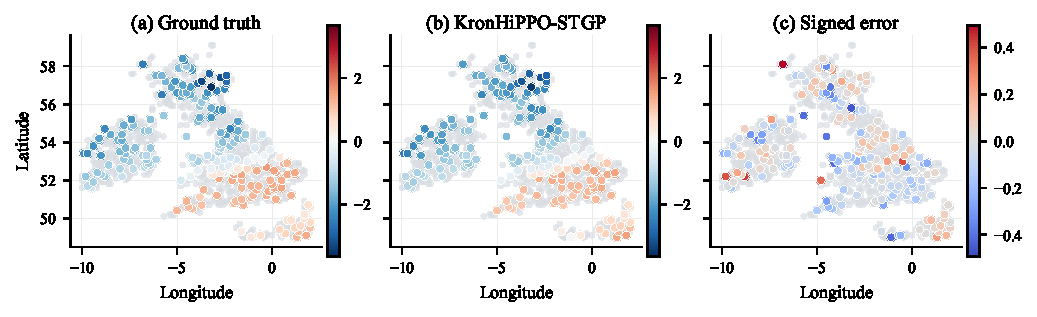
\includegraphics[width=0.98\textwidth]{figures/era5_long_tasks1_10_spatial_snapshot_horizontal.pdf}
\caption{ERA5-Land Tasks~1--10 long-stream spatial snapshot at the final online
block for the predeclared seed-0 split. The panels show the standardized target
field, the \method posterior mean, and the signed prediction error at the 200
held-out UK locations; the remaining 800 visible locations are shown in light
gray for spatial context. The map geometry is used only for visualisation.}
\label{app:era5-long-map}
\end{figure}
\FloatBarrier

\subsection{COVID-19}

The COVID-19 dataset contains 52 weekly jurisdiction-level hospital-admission series from the CDC NHSN Hospital Respiratory Data release \citep{CDCWeeklyHospitalization}. The target is the standardised $\log(1+x)$ transform of weekly confirmed COVID-19 admissions per 100,000 population.
Task~1 provides the initial 52-week calibration period, followed by 143 weeks
processed strictly online. Each formal split observes 42
jurisdictions and predicts 10 held-out jurisdictions before their labels are
revealed. The composite figure uses the predeclared seed-5 Connecticut and
Nevada trajectories, selected by the largest distance between z-scored
observed trajectories among the four archived candidates.

\begin{figure}[!t]
\centering
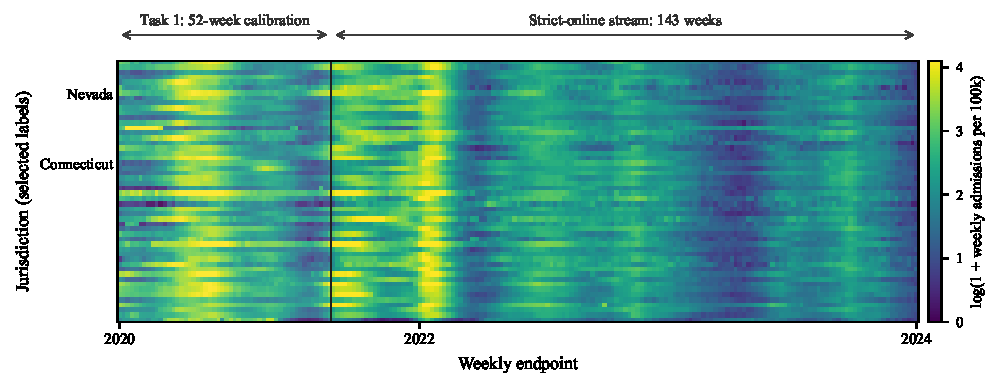
\includegraphics[width=0.96\textwidth]{figures/dataset_overview_covid_heatmap.pdf}
\vspace{3pt}

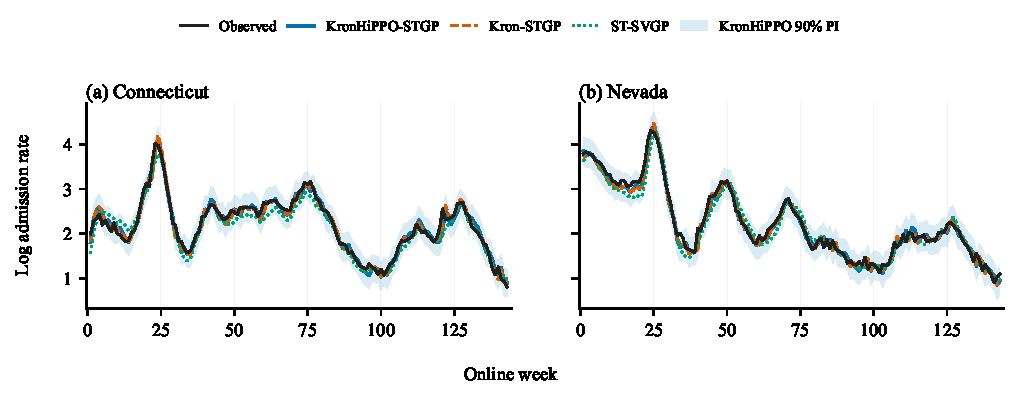
\includegraphics[width=0.96\textwidth]{figures/fig_covid_trajectories_side_by_side.pdf}
\caption{COVID-19 dataset structure and replay-free qualitative evidence. The
upper panel shows the jurisdiction-by-week overview, with the 52-week calibration
period separated from the subsequent 143-week strict-online stream. The lower
panels show seed-5 Connecticut and Nevada trajectories selected by the archived
observed-trajectory diversity rule; a shared y-scale and legend are used for the
same predictive methods in both jurisdictions.}
\label{app:covid-composite}
\end{figure}

\FloatBarrier

\subsection{PEMS-BAY}

PEMS-BAY contains traffic-speed measurements from 325 Bay Area sensors sampled every five minutes in the public DCRNN benchmark release \citep{Li2018DCRNN}. We use the
data for contemporaneous spatial nowcasting rather than future traffic
forecasting. In each formal split, 260 sensors are visible and 65 are held out,
with held-out labels revealed only after prediction. The protocol uses
$M_s=32$, $M_t=128$, 512 random Fourier features, and the locked road-context
X-lag mean design. All nine matched mechanism runs complete without OOM or
divergence.
Figure~\ref{fig:representative-replay-free} uses the predeclared seed-1 sensors
nearest the 15th, 50th, and 85th percentiles of full-stream \method RMSE:
sensors 400952, 400965, and 400178, respectively. Sensor selection therefore
follows the predefined \method difficulty quantiles. The common 48-hour plotting
window is selected independently using observed speeds only, by maximising the
median held-out speed range; the relative performance of the displayed methods
is not used for window selection.

\begin{figure}[!t]
\centering
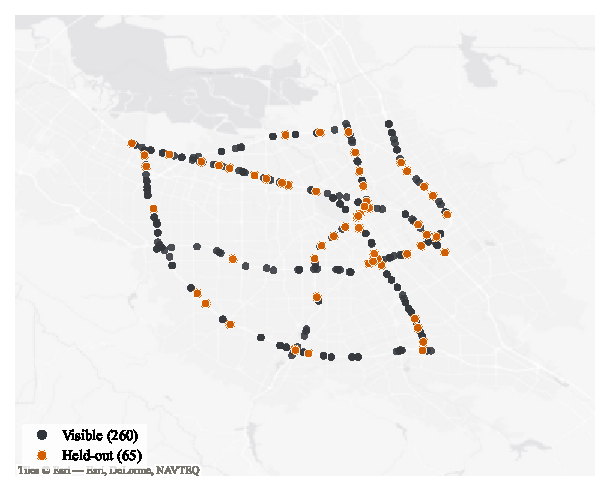
\includegraphics[width=0.78\textwidth]{figures/dataset_overview_pems.pdf}
\caption{PEMS-BAY sensor geometry for the archived seed-0 spatial split.
Dark-gray points are visible sensors and orange points are held-out sensors,
shown over a pale Bay Area road basemap. The geometry is used only to
visualise the contemporaneous held-out-sensor protocol. Map attribution is
included in the artwork.}
\label{app:pems-map}
\end{figure}

\subsection{Mechanism and transfer diagnostics}

Within each dataset, the joint/changing and zero-cross/changing variants share the same split, calibration, inducing-variable budgets, and changing inducing-representation maps. Zero-cross removes the accumulated trend--residual likelihood cross block after the transported historical and current-block statistics are combined. Joint/fixed-global uses complete-horizon temporal inducing representations and is reported separately as an offline representation reference.

The transfer diagnostic evaluates a separate mechanism by comparing the transported online state with a finite-dimensional variational reference posterior recomputed from the observed history in the current inducing representation. We report the marginal predictive Gaussian KL $\mathrm{KL}(p_{\mathrm{online}}\|p_{\mathrm{reference}})$, averaged first over query locations within each non-warm-up block, then over blocks within each seed, and finally across seeds. At $M_t=128$, the reported value $1.27\times10^{-4}$ is this aggregated diagonal predictive KL; it is neither a joint-output KL nor a solver residual. The solver benchmark instead uses identical positive-definite systems and right-hand sides for dense and structured posterior solves, thereby isolating numerical solution from representation transfer.

For each solver size, dense and structured posterior solves are evaluated on the same matched random systems. The displayed dense and structured runtimes are means, whereas speed-up is computed within each replicate as $t_{\mathrm{dense}}/t_{\mathrm{structured}}$ before averaging across replicates. The resulting mean speed-up therefore need not equal the ratio of the two displayed mean runtimes.
Figure~\ref{fig:main-mechanism} (c) visualises this matched solver benchmark, while Table~\ref{tab:solver} reports selected runtimes, paired speed-ups, and relative solution errors.

The lower off-diagonal block is reconstructed as the transpose when assembling the symmetric precision; all other retained statistics and assimilation steps remain unchanged. Because the removed block contains both historical and current-block contributions, the ablation tests joint likelihood coupling rather than historical trend revision alone.

Operating-point robustness. We repeat the zero-cross intervention under the archived ERA5 setting used in Table~1, without retuning either arm, to test whether the result depends on the spectral-mixture mechanism configuration. The full run reproduces the archived predictive means and variances to numerical precision (maximum absolute differences $4.23\times10^{-12}$ and $5.15\times10^{-15}$), while zero-cross again degrades every point and proper scoring-rule metric. Complete results are reported in Table~\ref{tab:mechanism_full}.

\begin{center}
\captionof{table}{Full mechanism results and ERA5 operating-point robustness check (mean $\pm$ sample SD). The first two blocks report the formal ERA5-Land and PEMS-BAY mechanism suites; the final block repeats the joint-versus-zero-cross intervention under the Table-1 ERA5 configuration. Coverage90 provides an additional calibration diagnostic.}
\label{tab:mechanism_full}
\small
\setlength{\tabcolsep}{4.0pt}
\begin{tabular}{@{}lrrrrr@{}}
\toprule
Variant & RMSE $\downarrow$ & CRPS $\downarrow$ & NLPD $\downarrow$ & ECE $\downarrow$ & Coverage90 \\
\midrule
\multicolumn{6}{@{}l}{\textit{ERA5-Land (five 171-block runs)}} \\
Joint / changing & $0.1251\pm0.0034$ & $0.0665\pm0.0014$ & $-0.6837\pm0.0186$ & $0.0461\pm0.0029$ & $0.9134\pm0.0035$ \\
Zero-cross / changing & $1.2898\pm0.0120$ & $0.9951\pm0.0088$ & $52.8139\pm1.9682$ & $0.6905\pm0.0018$ & $0.1148\pm0.0019$ \\
Joint / fixed-global & $0.1950\pm0.0030$ & $0.1420\pm0.0009$ & $0.2580\pm0.0043$ & $0.1807\pm0.0012$ & $0.9933\pm0.0006$ \\
\addlinespace[1pt]
\cmidrule(lr){1-6}
\addlinespace[1pt]
\multicolumn{6}{@{}l}{\textit{PEMS-BAY (three formal spatial splits)}} \\
Joint / changing & $0.7666\pm0.0629$ & $0.3774\pm0.0193$ & $1.1883\pm0.1076$ & $0.1317\pm0.0196$ & $0.9032\pm0.0204$ \\
Zero-cross / changing & $0.9555\pm0.0232$ & $0.4856\pm0.0123$ & $1.5333\pm0.1323$ & $0.0474\pm0.0132$ & $0.8490\pm0.0217$ \\
Joint / fixed-global & $0.8112\pm0.0665$ & $0.4092\pm0.0208$ & $1.2194\pm0.0637$ & $0.1760\pm0.0101$ & $0.9249\pm0.0112$ \\
\addlinespace[1pt]
\cmidrule(lr){1-6}
\addlinespace[1pt]
\multicolumn{6}{@{}l}{\textit{ERA5-Land (Table-1 operating point)}} \\
Joint / changing & $0.1416\pm0.0036$ & $0.0766\pm0.0017$ & $-0.3349\pm0.0434$ & $0.0669\pm0.0067$ & $0.7830\pm0.0089$ \\
Zero-cross / changing & $1.2921\pm0.0127$ & $1.0142\pm0.0090$ & $97.1323\pm2.8269$ & $0.4599\pm0.0007$ & $0.0841\pm0.0013$ \\
\bottomrule
\end{tabular}
\end{center}

\begin{center}
\captionof{table}{Coordinate-transfer control at $M_t=128$ (mean $\pm$ sample SD over five spatial splits). Predictive KL is $\mathrm{KL}(p_{\mathrm{online}}\Vert p_{\mathrm{reference}})$ against the finite-dimensional variational reference posterior recomputed in the current inducing representation. Identity reuse changes only the historical likelihood transfer; all current-representation model and inference components are held fixed. Coverage90 has a nominal target of $0.90$.}
\label{tab:coordinate_control}
\small
\setlength{\tabcolsep}{10pt}
\begin{tabular}{@{}lcc@{}}
\toprule
Metric & Conditional transport & Identity reuse \\
\midrule
Predictive KL $\downarrow$ & $1.2649\times10^{-4}\pm5.9122\times10^{-6}$ & $2.0713\pm0.1158$ \\
RMSE $\downarrow$ & $0.0795\pm0.0051$ & $0.2651\pm0.0024$ \\
CRPS $\downarrow$ & $0.0463\pm0.0017$ & $0.1520\pm0.0015$ \\
NLPD $\downarrow$ & $-0.9687\pm0.0251$ & $1.0741\pm0.0960$ \\
ECE $\downarrow$ & $0.1913\pm0.0085$ & $0.1604\pm0.0055$ \\
Coverage90 & $0.9825\pm0.0038$ & $0.6320\pm0.0074$ \\
\bottomrule
\end{tabular}
\end{center}

\begin{center}
\captionof{table}{Dense versus Schur--Sylvester posterior solves on matched systems. Runtimes are reported as means; speed-up is the mean of the within-replicate $t_{\mathrm{dense}}/t_{\mathrm{structured}}$ ratios and therefore need not equal the ratio of the mean runtimes. Relative error is measured against the dense solution.}
\label{tab:solver}
\small
\setlength{\tabcolsep}{7pt}
\begin{tabular}{@{}lrrrr@{}}
\toprule
$M_s=M_t$ & Dense (ms) & Structured (ms) & Speed-up $\uparrow$ & Rel. error $\downarrow$ \\
\midrule
16 & $1.072$ & $0.137$ & $7.9\times$ & $9.2\times10^{-14}$ \\
32 & $27.919$ & $0.403$ & $69.6\times$ & $9.1\times10^{-13}$ \\
64 & $994.822$ & $0.974$ & $1036.7\times$ & $4.7\times10^{-12}$ \\
\bottomrule
\end{tabular}
\end{center}

\begin{center}
\centering
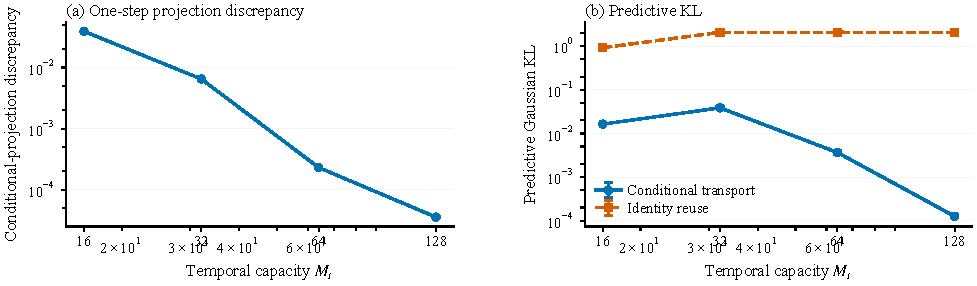
\includegraphics[width=0.98\textwidth]{figures/mechanism_diagnostics_two_panel.pdf}
\captionof{figure}{Transfer diagnostics. (a) One-step conditional-projection discrepancy. (b) Predictive Gaussian KL to the current-representation reference across temporal capacities for conditional transport and identity reuse. Conditional transport is non-monotone across the sweep, while identity reuse remains at order-one KL for $M_t\ge32$.}
\label{fig:transfer_solver_diagnostics}
\end{center}

\FloatBarrier
\clearpage

\subsection{Implementation efficiency audit}

The archived short-batch implementation audit at
$M_s=M_t=128$ on an RTX~4090 reports the ST-SVGP and KronHiPPO-STGP accuracy,
training wall time, profiler count, and peak reserved GPU memory from the same
audit record. This is an implementation-level comparison rather
than a framework-neutral complexity benchmark: the profiler column reports
supported-operation counts from the corresponding implementations and does not
represent complete hardware instruction-level FLOPs. The reported $40.4\times$
difference is therefore interpreted as a profiler-count ratio, while the
wall-clock and peak-memory ratios are measured implementation outcomes.

\begin{center}
\captionof{table}{Archived ERA5 short-batch implementation audit at $M_s=M_t=128$ on an RTX~4090. Accuracy and efficiency entries within each row come from the same audit record. \texttt{Train} denotes recorded training wall time, \texttt{Profiler GFLOPs/step} denotes supported-operation profiler counts, and \texttt{Peak} denotes reserved GPU memory.}
\label{tab:practical-efficiency}
\resizebox{0.82\textwidth}{!}{%
\begin{tabular}{@{}lrrrr@{}}
\toprule
Method & RMSE & Train (s) & \shortstack{Profiler\\GFLOPs/step} & Peak (GiB) \\
\midrule
ST-SVGP & 0.0837 & 4,586.83 & 1,106.04 & 14.75 \\
\method & 0.0882 & 41.39 & 27.36 & 1.68 \\
\midrule
\textit{Relative difference} & $+5.4\%$ RMSE & $110.8\times$ faster & $40.4\times$ lower & $8.8\times$ lower \\
\bottomrule
\end{tabular}
}
\end{center}

Appendix Table~\ref{app:efficiency-online} reports a separate strict-online accounting over Tasks~2--10, including
end-to-end execution, per-block posterior-update latency, prediction time, GPU
memory, and persistent-state size. These online records use a different
measurement scope from the short-batch audit and are therefore not combined with
Table~\ref{tab:practical-efficiency}
to form a cross-hardware or architecture-independent speed ratio.

\begin{center}
\captionof{table}{Online efficiency summary for ERA5 Tasks~2--10 using the formal
method names. End-to-end timing includes the online blocks, while the GPU and
persistent-state columns are implementation-specific. These values should not
be interpreted as hardware-normalised cross-method speed ratios.}
\label{app:efficiency-online}
\small
\setlength{\tabcolsep}{5.0pt}
\begin{tabular}{@{}lrrrrr@{}}
\toprule
Method & End-to-end (s) & Iter./block (s) & Predict (s) & GPU MiB & State MiB \\
\midrule
OSGPR & 78.00 & 0.1923 & 20.270 & 657 & 0.25 \\
StreamingSGPR & 29.81 & 0.0336 & 1.414 & 816 & 0.25 \\
Official OHSVGP & 254.32 & 1.2312 & 12.398 & 1966 & 0.08 \\
\method & 79.52 & 0.0214 & 3.562 & 1067 & 19.16 \\
Kron-STGP & 61.06 & 0.0204 & 3.500 & 1069 & 20.92 \\
\bottomrule
\end{tabular}
\end{center}
\FloatBarrier
